% Chapter 6 from the standard thesis template
%  Conclusions and Future work
\chapter{Conclusion and Future work} 

\section{Conclusion}
In this thesis we have shown that an off the shelf SDR can be used to perform as a radiometer.  Using a SDR has several advantages such as a more flexible system and can result in a less expensive system.  Since a SDR offers high flexibility, changes to the system can be done very quickly and helps in future proofing the system.  Since off the shelf components were used, it also allowed for a lower cost system that is able to perform variations of power detection in a radiometer without adding more costly RF components.  Finally, this type of radiometer is very flexible and allows for it to adapt to possible changing conditions.  This again happens with no change to the RF hardware and instead happens within the software of the system.

\section{Future work}
The main purpose of this research is to demonstrate and prove that an off the shelf software defined radio is capable of operating like a radiometer and can do so within the same or better specifications that are seen in most radiometers today.  To do that, we used a very basic radiometer setup and configured our SDR to behave as a single input radiometer.  It was also assumed that the input from the RF front end of the radiometer was stable, which in our case was accomplished by stabilizing the temperature of the active components in the RF Front end.

However, this temperature stabilization requires extra weight and bulk to be added to the radiometer.  In the application that the ISU radiometer was designed for, this was not a major drawback to the system.  However other applications may require a system that does not have this type of temperature stabilization.  For those type of systems, other radiometers use different methods to account for and adjust for fluctuations in the RF front end. 

\subsection{Improving on the FPGA firmware}

For this thesis we focused on the software that would run on a PC or comparable computer system running a full OS like Linux.  While this aids to speed up development and works just fine for testing the theory on a off the shelf SDR acting as a radiometer, it does require additional hardware.  For some applications of a radiometer, this is not a huge concern.  In the case for the ISU radiometer, the concern is not that large since the radiometer is not designed to be "portable" and requires additional support equipment such as a generator anyway.  However, other remote sensing applications, such as space based applications, would require a more efficient method.  It is very possible to move the software generated in GNURadio into the firmware of the N200.  This will help to offload the work needed by the computer and would allow for the computer or similar system to act as more of a control method and for data storage.  

\subsection{Correlation}  
One such method is to correlate the information with another input which can be another antenna looking at the same source or can be two polarization from the same antenna.  This results in two receiver systems looking at the same source and you have two signals, $S_1$ and $S_2$.  Since we are looking at the same source, both signals will be correlated in time, and when multiplied they will provide an output proportional to the strength of the source signal.  The noise introduced by each receiver will then have a lower correlation due to the random nature of the noise.  This results in a radiometer with a greater sensitivity due to the reduction of the noise even though two receivers are used [\cite{Fujimoto}].

The N200 software defined radio was chosen as it is capable of having two different daughter-cards plugged in.  Therefore it is possible to have both sources enter the software defined radio and once digitized we can sum the magnitudes of the two incoming sources.  This is quite easy to do and is shown in figure \ref{correlating_sdr}.

{\begin{figure}[h!tb] 
\centering
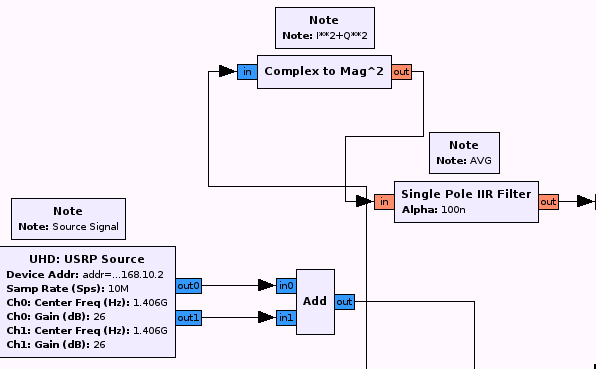
\includegraphics[width=14cm]{Images/N200_rad_corr.png}
\isucaption{The key blocks used for creating a correlating radiometer in software.  The key blocks is the USRP source, which allows us to address both daughter-boards and the ADD block which sums the signals.}
\label{correlating_sdr}
\end{figure}
}

Although figure \ref{correlating_sdr} shows a correlating software defined radio radiometer, it has not been tested.  In theory, this should correlate the signal and improve the sensitivity of the radiometer, however further testing is needed.

\subsection{Improving stability with a feedback loop}

One of the largest challenges with a radiometer is improving the stability of the radiometer.  Drifts in temperature can greatly affect the gains from the LNAs and also change how much noise all of the components in the radiometer contribute.  A software defined radio can help as we are digitizing the signal as soon as possible.  This helps in eliminating the analog components for power detection and even for filtering, but does not eliminate all of the physical hardware, mainly the LNAs.  In this thesis, we did not focus on this issue since the RF front end of the ISU radiometer is temperature controlled.  All components are mounted to an aluminum block which is attached to a thermal electric cooler.  This system then maintains the temperature within 1 degree C.  

However a more compact, lower cost and easier setup would be to just have the LNAs attach directly to the SDR without any temperature compensation.  While this can be done, we have now lost stability in the LNAs and we need to compensate for that.  One method that is discussed by William Goggins is to use a feedback loop to continuously adjust a variable attenuator [\cite{Goggins}].  In Goggins paper, he discusses using a servo that mechanically controls the attenuator.  However since we are in the digital domain, we can control this all in software, and doing a feedback loop is quite easy for a computer to do.  